% Tipo de documento y otras especificaciones
\documentclass[12pt,letterpaper]{article}
% Configuracion
% Para escribir tildes y eñes
\usepackage[utf8]{inputenc}

% Para que los títulos de figuras, tablas y otros estén en español
\usepackage[spanish]{babel} 

% Los paquetes ams son desarrollados por la American Mathematical Society y mejoran la escritura de fórmulas y símbolos matemáticos.
\usepackage{amsmath}
\usepackage{amsfonts}
\usepackage{amssymb}

% Para insertar gráficas
\usepackage{graphicx}

% Para colocar varias figuras
\usepackage[lofdepth,lotdepth]{subfig}

% Para la presentación correcta de unidades
\usepackage{unitsdef}

% Redimensionamiento del espacio entre magnitud y unidad
\renewcommand{\unitvaluesep}{\hspace*{4pt}}

% Para insertar hipervínculos y marcadores
\usepackage[colorlinks=true,urlcolor=blue,linkcolor=black,citecolor=green]{hyperref}

% Para ubicar las tablas y figuras justo después del texto
\usepackage{float}

% Para hacer tablas más estilizadas
\usepackage{booktabs}

% Para manejar los encabezados y pies de página
\usepackage{fancyhdr}

% Cambiar nombre a tablas
\addto\captionsspanish{\renewcommand{\tablename}{Tabla}}
% Cambiar nombre a lista de tablas
\addto\captionsspanish{\renewcommand{\listtablename}{Índice de tablas}}

% Tamaño del área de escritura de la página
\usepackage[left=18mm,right=18mm,top=21mm,bottom=21mm]{geometry}

%Codigo
\usepackage{listings}
\usepackage{xcolor}

% Definicion de colores
\definecolor{codegreen}{rgb}{0,0.6,0}
\definecolor{codegray}{rgb}{0.5,0.5,0.5}
\definecolor{codepurple}{rgb}{0.58,0,0.82}
\definecolor{backcolour}{rgb}{0.95,0.95,0.92}

\lstdefinestyle{mystyle}{
    language=Python, % Specify the programming language
    backgroundcolor=\color{backcolour}, % Background color for the listing
    commentstyle=\color{codegreen}, % Comment style
    keywordstyle=\color{magenta}, % Keyword style
    numberstyle=\tiny\color{codegray}, % Line number style
    stringstyle=\color{codepurple}, % String literal style
    basicstyle=\ttfamily\footnotesize, % Basic style
    breakatwhitespace=false, % Break lines only at whitespace
    breaklines=true, % Automatic line breaking
    captionpos=b, % Position of the caption
    keepspaces=true, % Keep spaces in the listing
    numbers=left, % Position of line numbers
    numbersep=5pt, % Padding between line numbers and code
    showspaces=false, % Show spaces with underscores?
    showstringspaces=false, % Show spaces in strings?
    showtabs=false, % Show tabs within strings?
    tabsize=2 % Tab size
}

\usepackage{lastpage}
\graphicspath{{./Figuras/}}
\pagenumbering{arabic}


% Contenido de los encabezados y pies de pagina
\pagestyle{fancy}
\lhead{IE0117: Programación Bajo Plataformas Abiertas}
\rhead{Reporte Laboratorio \#}
\lfoot{Escuela de Ingeniería Eléctrica}
\cfoot{\thepage\ de \pageref{LastPage}}
\rfoot{Universidad de Costa Rica}

\let\OLDthebibliography=\thebibliography
\def\thebibliography#1{\OLDthebibliography{#1}%
\addcontentsline{toc}{section}{\refname}}

\makeatletter
\renewcommand\@biblabel[1]{#1. \ }
\makeatother


\begin{document}

\begin{titlepage}

% Define un nuevo comando para las líneas horizontales, cambio de grosor
\newcommand{\HRule}{\rule{\linewidth}{0.5mm}}

% Centra todo en la página
\center

%----------------------------------------------------------------------------------------
%	SECCIONES DE ENCABEZADO
%----------------------------------------------------------------------------------------

% Nombre de la universidad
\textsc{\LARGE UNIVERSIDAD DE COSTA RICA}\\[1.5cm]
% Nombre de la escuela
\textsc{\Large Escuela de Ingeniería Eléctrica}\\[0.5cm]
% Título del curso
\textsc{\large IE0117: Programación Bajo Plataformas Abiertas}\\[0.5cm]

%----------------------------------------------------------------------------------------
%	SECCIÓN DE TÍTULO
%----------------------------------------------------------------------------------------
\bigskip
\bigskip
\bigskip
\bigskip

% Título del documento
\HRule \\[0.4cm]
{ \huge \bfseries Reporte\\[0.5cm] \LARGE Laboratorio \#}\\[0.4cm]
\HRule \\[1.5cm]

%----------------------------------------------------------------------------------------
%	SECCIÓN DE AUTOR
%----------------------------------------------------------------------------------------

\begin{center} \large
Prof. Carolina Trejos Quirós\\
\bigskip
\bigskip
\bigskip
\bigskip
Estudiante: Nombre Apellido, Carne
\end{center}
\bigskip
\bigskip
\bigskip
\bigskip
\bigskip
\bigskip
\bigskip
\bigskip
\bigskip
\bigskip
\bigskip
\bigskip
\bigskip
\bigskip
\bigskip
\bigskip
\normalsize \today \vspace*{5\baselineskip}
\vfill % Rellena el resto de la página con espacios en blanco

\end{titlepage}


\tableofcontents

\newpage

%----------------------------------------------------------------------------------------
%	INTRODUCCION
%----------------------------------------------------------------------------------------

\section{Introducción}

En esta sección se espera una introducción de las tareas realizadas en el laboratorio/proyecto. Al igual que el enlace del repositorio de Git donde se encuentra la implementación.

Ejemplo de \href{https://www.google.com}{link}.

%----------------------------------------------------------------------------------------
%	IMPLEMENTACION
%----------------------------------------------------------------------------------------

\section{Implementación}

En esta sección se debe incluir una explicación detallada de como abordaron los ejercicios del laboratorio/proyecto. Incluir los pasos tomados, algoritmos o técnicas utilizadas, diseños, fragmentos de código o pseudocódigo, entre otros. La idea es que el estudiante demuestre la comprensión del problema y de su solución.

\subsection{Figura}

\begin{figure}[h]
    \centering
    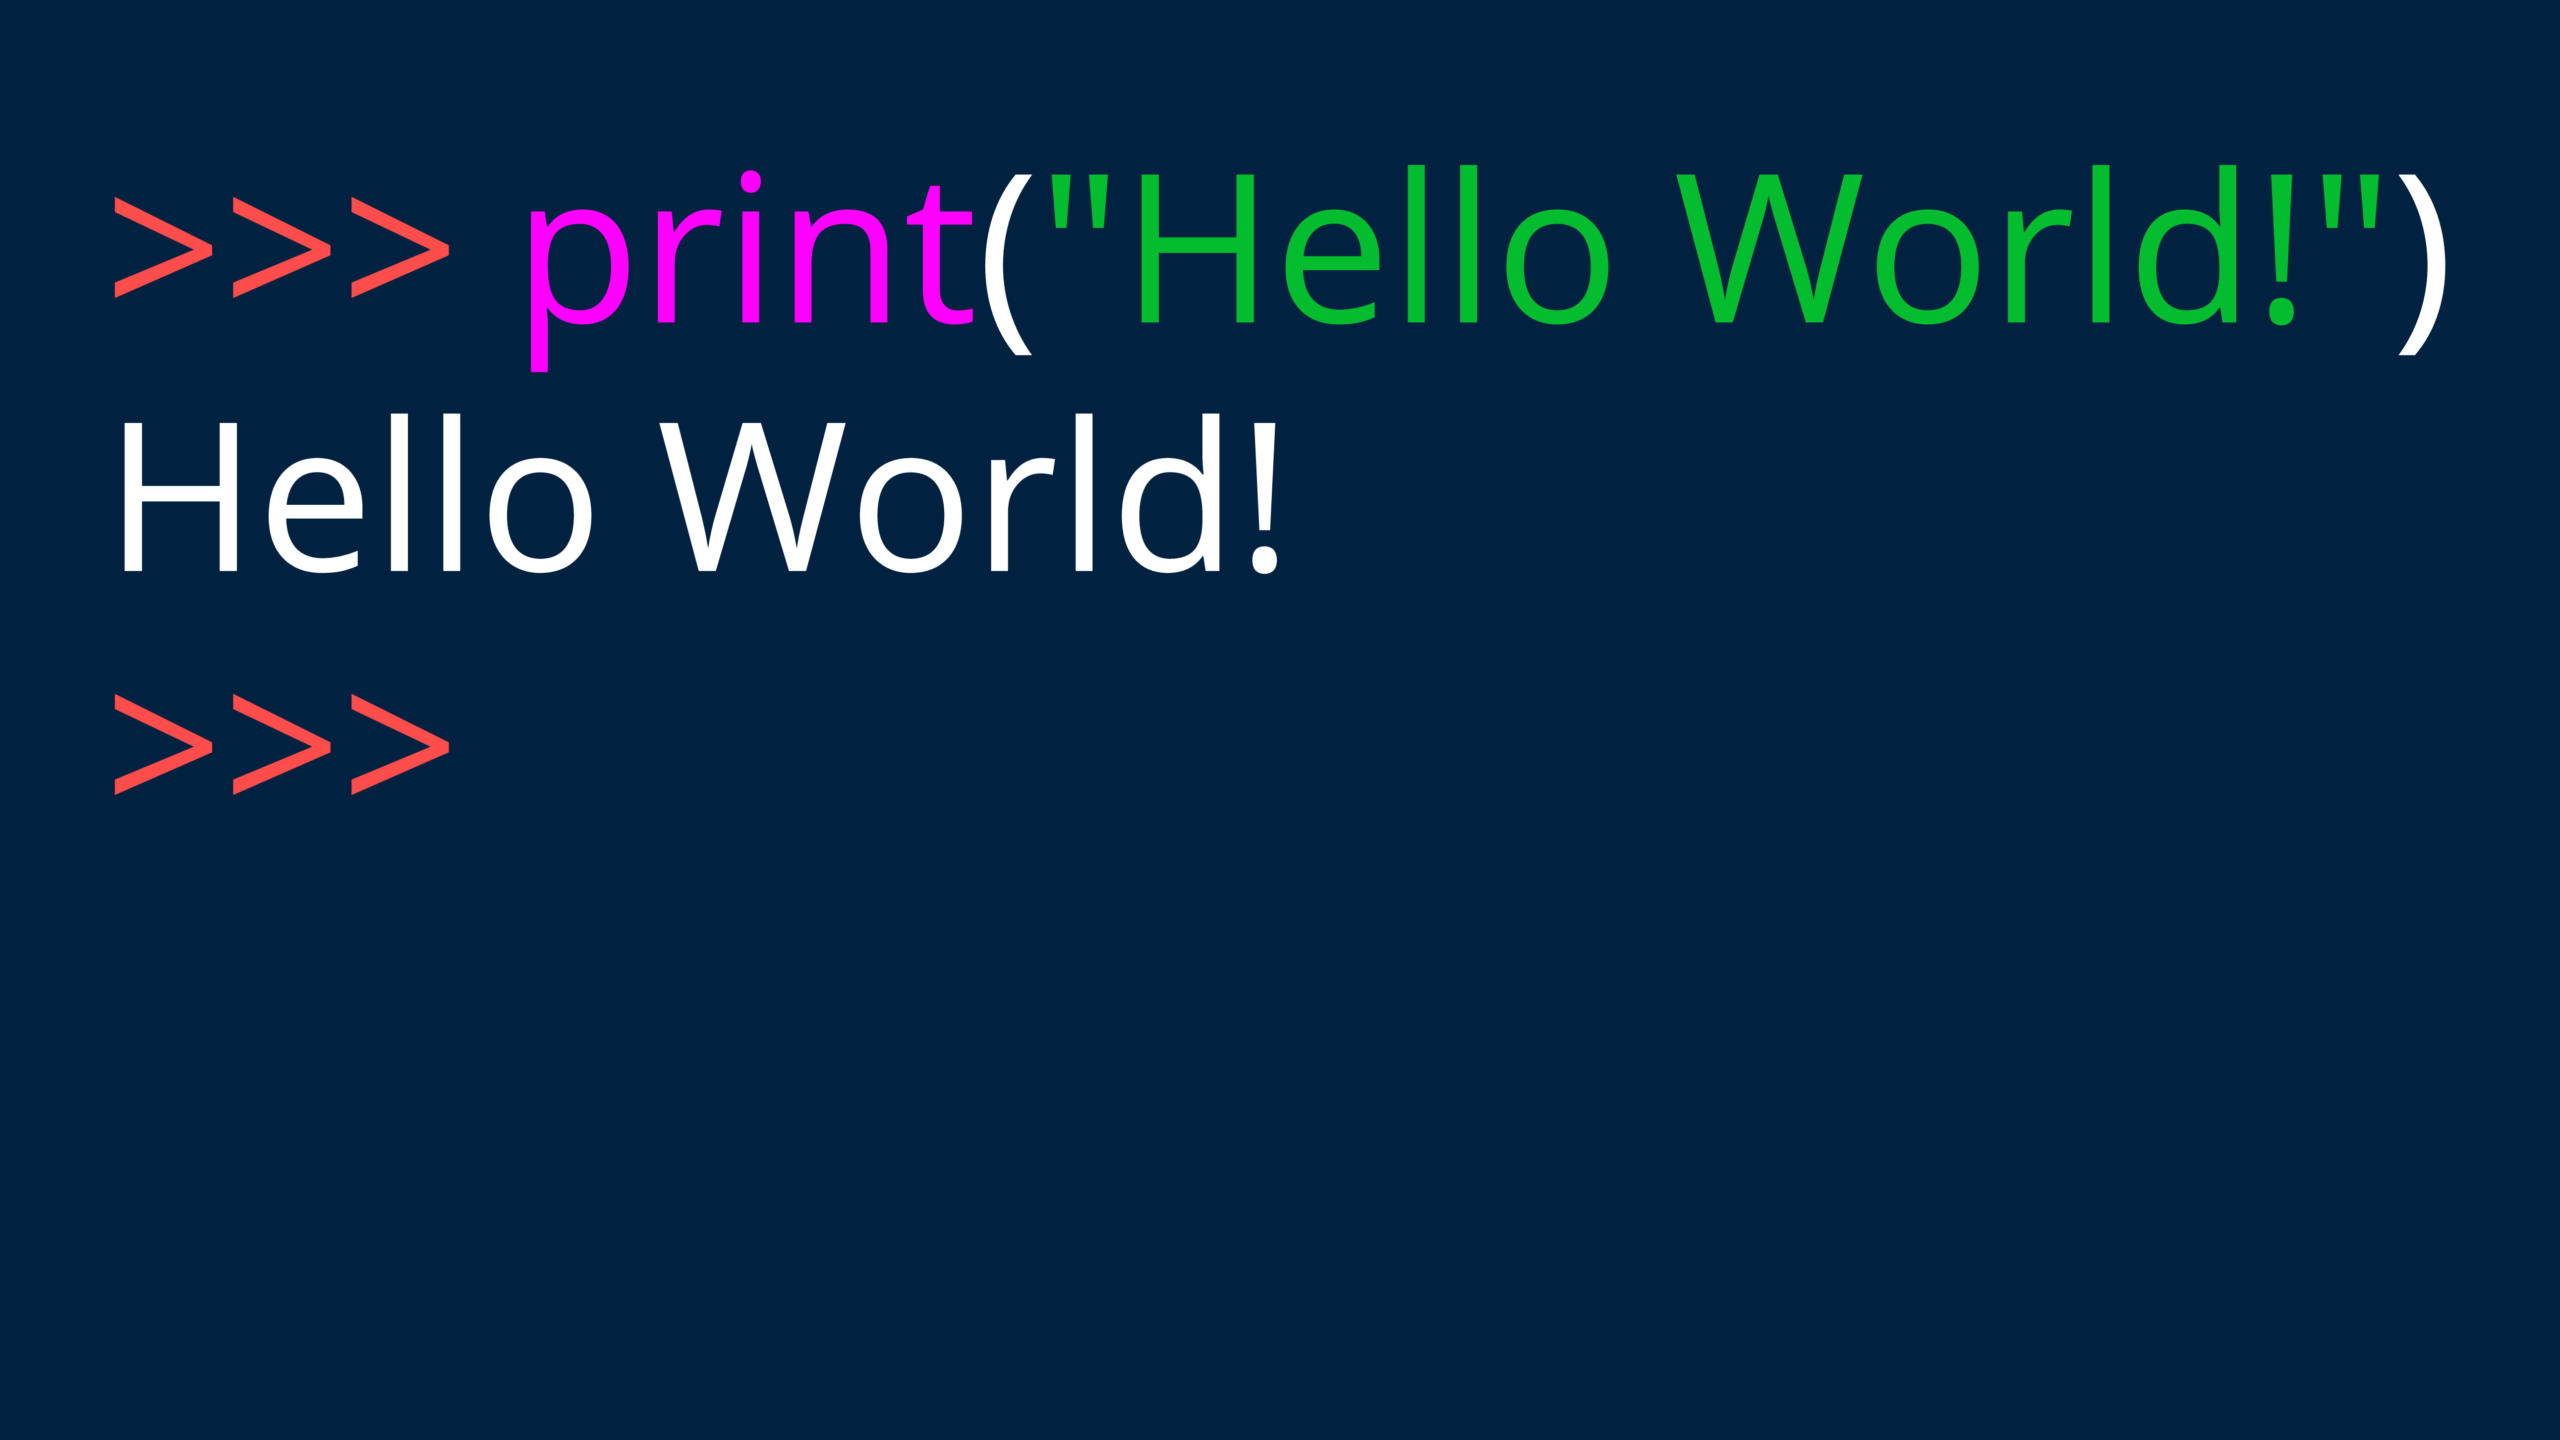
\includegraphics[scale=0.1]{Images/hello_world_py.jpeg}
    \caption{Ejemplo de imagen \cite{knuth:1984}.}
    \label{fig:ejemplo_imagen}
\end{figure}

Ejemplo de referencia de figuras \ref{fig:ejemplo_imagen}.

\subsection{Tabla}

\begin{table}[H]
\caption{Ejemplo tabla} \label{tab:ejemplo_tabla}
    \begin{center}
    	\begin{tabular}{@{}*{4}{c}@{}}
            \toprule
            $C_0$ & $C_1$\\
            \midrule
            1 & 2\\
        	3 & 4\\
        	\bottomrule
        \end{tabular}
    \end{center}
\end{table}

Ejemplo de referencia de tablas \ref{tab:ejemplo_tabla}.

\subsection{Ecuaciones}

\begin{equation} \label{eq:formula_triangulo}
    T_n = \frac{n(n+1)}{2}
\end{equation}

Ejemplo de referencia de ecuaciones \eqref{eq:formula_triangulo}.

\subsection{Código}

\begin{lstlisting}[style=mystyle, caption={Ejemplo de codigo}, label=lst:ejemplo_codigo]
def factorial(n):
    if n == 0:
        return 1
    else:
        return n * factorial(n-1)

result = factorial(5)
print("Factorial of 5 is:", result)
\end{lstlisting}

%----------------------------------------------------------------------------------------
%	RESULTADOS
%----------------------------------------------------------------------------------------

\section{Resultados}

En la sección de Resultados se debe incluir las pruebas realizadas sobre su código para corroborar su funcionalidad.

%----------------------------------------------------------------------------------------
%	CONCLUSIONES Y RECOMENDACIONES
%----------------------------------------------------------------------------------------

\section{Conclusiones y recomendaciones}

Finalmente, en esta sección resumir lo aprendido en el laboratorio/proyecto. Además, incluir los problemas que tuvo, como los resolvió y recomendaciones para el futuro.

\newpage
\clearpage

%----------------------------------------------------------------------------------------
%	BIBLIOGRAFIA
%----------------------------------------------------------------------------------------

\bibliographystyle{ieeetr}
\bibliography{references}

\end{document}
